\section{夹逼准则}
\begin{theorem}\label{theorem:函数极限.夹逼准则}
%@see: 《数学分析(第二版 上册)》(陈纪修) P76 定理3.1.3
%@see: 《高等数学(第六版 上册)》 P50 准则I'
设函数\(f,g,h\in\mathbb{R}^D\)满足\begin{itemize}
	\item \((\exists\rho>0)
	[0<\abs{x-x_0}<\rho \implies g(x) \leq f(x) \leq h(x)]\),
	\item \(\lim_{x \to x_0} g(x) = \lim_{x \to x_0} h(x) = A\),
\end{itemize}
则\(\lim_{x \to x_0} f(x) = A\).
\begin{proof}
对于\(\forall\epsilon>0\),
有\begin{gather*}
	\lim_{x \to x_0} h(x) = A
	\implies
	(\exists\delta_1>0)
	(\forall x\in\mathbb{R})
	\left[
		\begin{array}{rl}
			0<\abs{x-x_0}<\delta_1
			&\implies
			\abs{h(x)-A}<\epsilon \\
			&\implies
			h(x)<A+\epsilon
		\end{array}
	\right], \\
	\lim_{x \to x_0} g(x) = A
	\implies
	(\exists\delta_2>0)
	(\forall x\in\mathbb{R})
	\left[
		\begin{array}{rl}
			0<\abs{x-x_0}<\delta_2
			&\implies
			\abs{h(x)-A}<\epsilon \\
			&\implies
			A-\epsilon<g(x)
		\end{array}
	\right].
\end{gather*}
取\(\delta=\min\{\delta_1,\delta_2,\rho\}\),
则\[
	(\forall x\in\mathbb{R})
	[
		0<\abs{x-x_0}<\delta
		\implies
		A-\epsilon < g(x) \leq f(x) \leq h(x) < A+\epsilon
	],
\]
即\(\lim_{x \to x_0} f(x) = A\).
\end{proof}
\end{theorem}

\begin{remark}
%@see: 《数学分析(第二版 上册)》(陈纪修) P83
当函数极限是不定号无穷大时,夹逼定理不成立,即\[
	g(x) \leq f(x) \leq h(x)
	\land
	\lim g(x) = \lim h(x) = \infty
	\notimplies
	\lim f(x) = \infty.
\]
\end{remark}

\begin{example}[重要极限I]
%@see: 《高等数学(第六版 上册)》 P51
试证:\begin{equation}\label{equation:函数极限.重要极限1}
	\lim_{x\to0} \frac{\sin x}{x} = 1.
\end{equation}
\begin{proof}
如图所示,
\begin{center}
	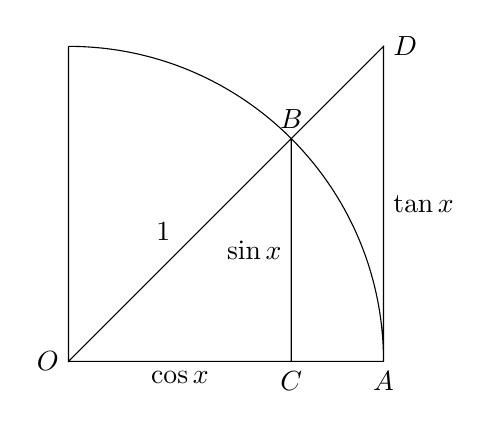
\begin{tikzpicture}
		\pgfmathsetmacro{\r}{4}
		\pgfmathsetmacro{\cx}{\r/sqrt(2)}
		\coordinate(O)at(0,0);
		\coordinate(A)at(\r,0);
		\coordinate(B)at(\cx,\cx);
		\coordinate(C)at(\cx,0);
		\coordinate(D)at(\r,\r);
		\draw (O)node[left]{\(O\)}
			--(C)node[below]{\(C\)}node[midway,below]{\(\cos x\)}
			--(A)node[below]{\(A\)}arc[start angle=0,end angle=90,radius=\r] (C)
			--(B)node[above]{\(B\)}node[midway,left]{\(\sin x\)}
			--(O)node[midway,above left]{\(1\)}
			--(0,\r)
			(B)
			--(D)node[right]{\(D\)}
			--(A)node[midway,right]{\(\tan x\)};
	\end{tikzpicture}
\end{center}
由于在\(0 < x < \pi/2\)时,\[
	0 < \sin x < x < \tan x
	\implies
	1 < \frac{x}{\sin x} < \frac{1}{\cos x}
	\implies
	\cos x < \frac{\sin x}{x} < 1.
\]
因为\(\lim_{x\to0}\cos x = 1\),
所以由\hyperref[theorem:数列极限.夹逼准则]{夹逼准则}可知,
\(\lim_{x\to0} \frac{\sin x}{x} = 1\).
\end{proof}
\end{example}

\begin{example}
计算极限\[
	\lim_{x\to0} \frac1x \sin\left(x^2 \sin\frac1x\right).
\]
\begin{solution}
%@see: https://www.bilibili.com/video/BV1FA4m1N7uv
因为\(0\leq\abs{\sin x}\leq\abs{x}\ (-\infty<x<+\infty)\),
所以\[
	0 \leq \abs{\sin\left(x^2 \sin\frac1x\right)}
	\leq \abs{x^2 \sin\frac1x}
	\leq \abs{x^2},
\]
从而\[
	0 \leq \abs{\frac1x \sin\left(x^2 \sin\frac1x\right)} \leq \abs{x}.
\]
因为\(\lim_{x\to0} \abs{x} = 0\),
所以由\hyperref[theorem:数列极限.夹逼准则]{夹逼准则}可知
\(\lim_{x\to0} \abs{\frac1x \sin\left(x^2 \sin\frac1x\right)} = 0\).
\end{solution}
\end{example}

\begin{example}
%@see: 《高等数学(第六版 上册)》 P56 习题1-6 4. (2)
证明:\(\lim_{n\to\infty} n \left(\frac1{n^2+\pi}+\frac1{n^2+2\pi}+\dotsb+\frac1{n^2+n\pi}\right)=1\).
\begin{proof}
易见\[
	\frac1{n^2+\pi}
	\geq \frac1{n^2+2\pi}
	\geq \dotsb
	\geq \frac1{n^2+n\pi},
\]
于是\[
	\frac{n}{n+\pi}
	\leq
	n \left(\frac1{n^2+\pi}+\frac1{n^2+2\pi}+\dotsb+\frac1{n^2+n\pi}\right)
	\leq
	\frac{n^2}{n^2+\pi}.
\]
因为\[
	\lim_{n\to\infty} \frac{n}{n+\pi}
	= \lim_{n\to\infty} \frac{n^2}{n^2+\pi}
	= 1,
\]
所以\(\lim_{n\to\infty} n \left(\frac1{n^2+\pi}+\frac1{n^2+2\pi}+\dotsb+\frac1{n^2+n\pi}\right)=1\).
\end{proof}
\end{example}

\begin{example}
%@see: 《高等数学(第六版 上册)》 P57 习题1-6 4. (4)
证明:\(\lim_{x\to0} \sqrt[n]{1+x} = 1\).
\begin{proof}
函数\(\sqrt[n]{1+x}\)的定义域是\(\Set{ x \given 1+x\geq 0 } = [-1,+\infty)\).

当\(x > 0\)时,
因为\(1 < \sqrt[n]{1+x} < 1+x\),
且\(\lim_{x\to0^+} 1 = \lim_{x\to0^+}(1+x) = 1\),
所以\[
	\lim_{x\to0^+} \sqrt[n]{1+x} = 1.
\]

当\(-1 < x < 0\)时,
因为\(1+x < \sqrt[n]{1+x} < 1\),
且\(\lim_{x\to0^-} 1 = \lim_{x\to0^-}(1+x) = 1\),
所以\[
	\lim_{x\to0^-} \sqrt[n]{1+x} = 1.
\]

综上,\(\lim_{x\to0} \sqrt[n]{1+x} = 1\).
\end{proof}
\end{example}

\begin{example}
%@see: 《高等数学(第六版 上册)》 P57 习题1-6 4. (5)
证明:\(\lim_{x\to0^+} x \floor*{\frac1x} = 1\).
\begin{proof}
令\(t=1/x\),
那么\[
	x \floor*{\frac1x} = \frac{1}{t} \floor{t}.
\]
又因为\[
	t - 1 < \floor{t} \leq t,
\]\[
	1 - \frac{1}{t} < \frac{1}{t} \floor{t} \leq 1;
\]
而\[
	\lim_{t\to+\infty} 1 - \frac{1}{t} = 1,
	\quad
	\lim_{t\to+\infty} 1 = 1,
\]
所以\[
	\lim_{x\to0^+} x \floor*{\frac1x} = \lim_{t\to+\infty} \frac{1}{t} \floor{t} = 1.
	\qedhere
\]
\end{proof}
\end{example}

%TODO: 函数\(\frac{\sin x}{x}\)的图像
% \begin{figure}[ht]
% 	\centering
% 	\begin{tikzpicture}
% 		\begin{axis}[
% 			xmin=-4*pi,xmax=4*pi,
% 			ymin=-.5,ymax=1.2,
% 			width=\textwidth,
% 			height=.3\textheight,
% 			grid=both,
% 			xlabel=$x$,
% 			ylabel=$y$,
% 			enlargelimits,
% 			axis lines=middle,
% 			xtick={3.14,6.28,9.42,-3.14,-6.28,-9.42},
% 			xticklabels={$\pi$,$2\pi$,$3\pi$,$-\pi$,$-2\pi$,$-3\pi$},
% 		]
% 			\begin{scope}[samples=50,thick,red]
% 				\addplot[domain=.01:4*pi]{sin(deg(x))/x};
% 				\addplot[domain=-4*pi:-.01]{sin(deg(x))/x};
% 			\end{scope}
% 			\filldraw[draw=black,fill=white](0,1)circle(1pt);
% 		\end{axis}
% 	\end{tikzpicture}
% 	\caption{函数\(y=\frac{\sin x}{x}\)的图像}
% 	\label{figure:极限.函数[y=sin(x)/x]的图像}
% \end{figure}

\begin{example}[重要极限II]
%@see: 《高等数学(第六版 上册)》 P53
试证:\begin{equation}\label{equation:函数极限.重要极限2}
	\lim_{x\to\infty} \left(1+\frac1x\right)^x = e.
\end{equation}
\begin{proof}
在\cref{section:极限.无理数e}我们已经知道,
数列\(x_n = \left(1+\frac1n\right)^n\)单调增加且有上界,收敛于\(e\).

当\(n\geq1\)时,
对于\(\forall x\in[n,n+1)\),
必有\[
	\left(1+\frac1{n+1}\right)^n
	< \left(1+\frac1x\right)^x
	< \left(1+\frac1n\right)^{n+1},
\]
且当\(n\to\infty\)时,
\(x\to+\infty\),
而\[
	\lim_{n\to\infty} \left(1+\frac1{n+1}\right)^n
	= \lim_{n\to\infty} \frac{\left(1+\dfrac1{n+1}\right)^{n+1}}{1+\dfrac1{n+1}}
	= \frac{\lim\limits_{n\to\infty} \left(1+\dfrac1{n+1}\right)^{n+1}}{\lim\limits_{n\to\infty} \left(1+\dfrac1{n+1}\right)}
	= \frac{e}1
	= e,
\]\[
	\lim_{n\to\infty} \left(1+\frac1n\right)^{n+1}
	= \lim_{n\to\infty} \left[\left(1+\frac1n\right)^n\cdot\left(1+\frac1n\right)\right]
	= \lim_{n\to\infty} \left(1+\frac1n\right)^n \cdot \lim_{n\to\infty} \left(1+\frac1n\right)
	= e \cdot 1
	= e,
\]
应用\hyperref[theorem:函数极限.夹逼准则]{夹逼准则}可得\[
	\lim_{x\to+\infty} \left(1+\frac1x\right)^x = e.
\]
令\(x=-(t+1)\),
则\(x\to-\infty\)时,
\(t\to+\infty\),
从而\begin{align*}
	\lim_{x\to-\infty} \left(1+\frac1x\right)^x
	&= \lim_{t\to+\infty} \left(1-\frac{1}{t+1}\right)^{-(t+1)}
	= \lim_{t\to+\infty} \left(\frac{t}{t+1}\right)^{-(t+1)} \\
	&= \lim_{t\to+\infty} \left(1+\frac1t\right)^{t+1}
	= \lim_{t\to+\infty} \left[\left(1+\frac1t\right)^t\cdot\left(1+\frac1t\right)\right]
	= e.
\end{align*}

综上所述,根据\cref{theorem:函数极限.极限与单侧极限的关系2},
由于\[
	\lim_{x\to+\infty}\left(1+\frac1x\right)^x
	= \lim_{x\to-\infty}\left(1+\frac1x\right)^x
	= e,
\]
所以\[
	\lim_{x\to\infty} \left(1+\frac1x\right)^x = e.
	\qedhere
\]
\end{proof}
\end{example}
